\documentclass{beamer}

\usepackage[utf8]{inputenc}
\usepackage[T1]{fontenc}

% \documentclass{beamer}
% \usepackage{amsmath}
% \usepackage{rotating}
% \usepackage{graphicx}
% \usepackage{multimedia}

% \useinnertheme[shadow=true]{rounded}
% \useoutertheme{shadow}
% \usecolortheme{orchid}
% \usecolortheme{whale}

% \mode<presentation>

% \newcommand{\dif}{\, \mathrm{d}}
% \newcommand{\diff}[2]{\frac{\mathrm{d}#1}{\mathrm{d}#2}}
% \newcommand{\partdiff}[2]{\frac{\partial #1}{\partial #2}}


% \title{TMA4280 - Introduction to supercomputing}
% \subtitle{Curriculum}
% \author{Arne Morten Kvarving}
% \institute{SINTEF ICT / NTNU}
% \date{January 2014}

% \begin{document}

% \maketitle
% \begin{frame}\frametitle{A short introduction to supercomputer history and
%                          hardware architecture}
% \begin{center}
% 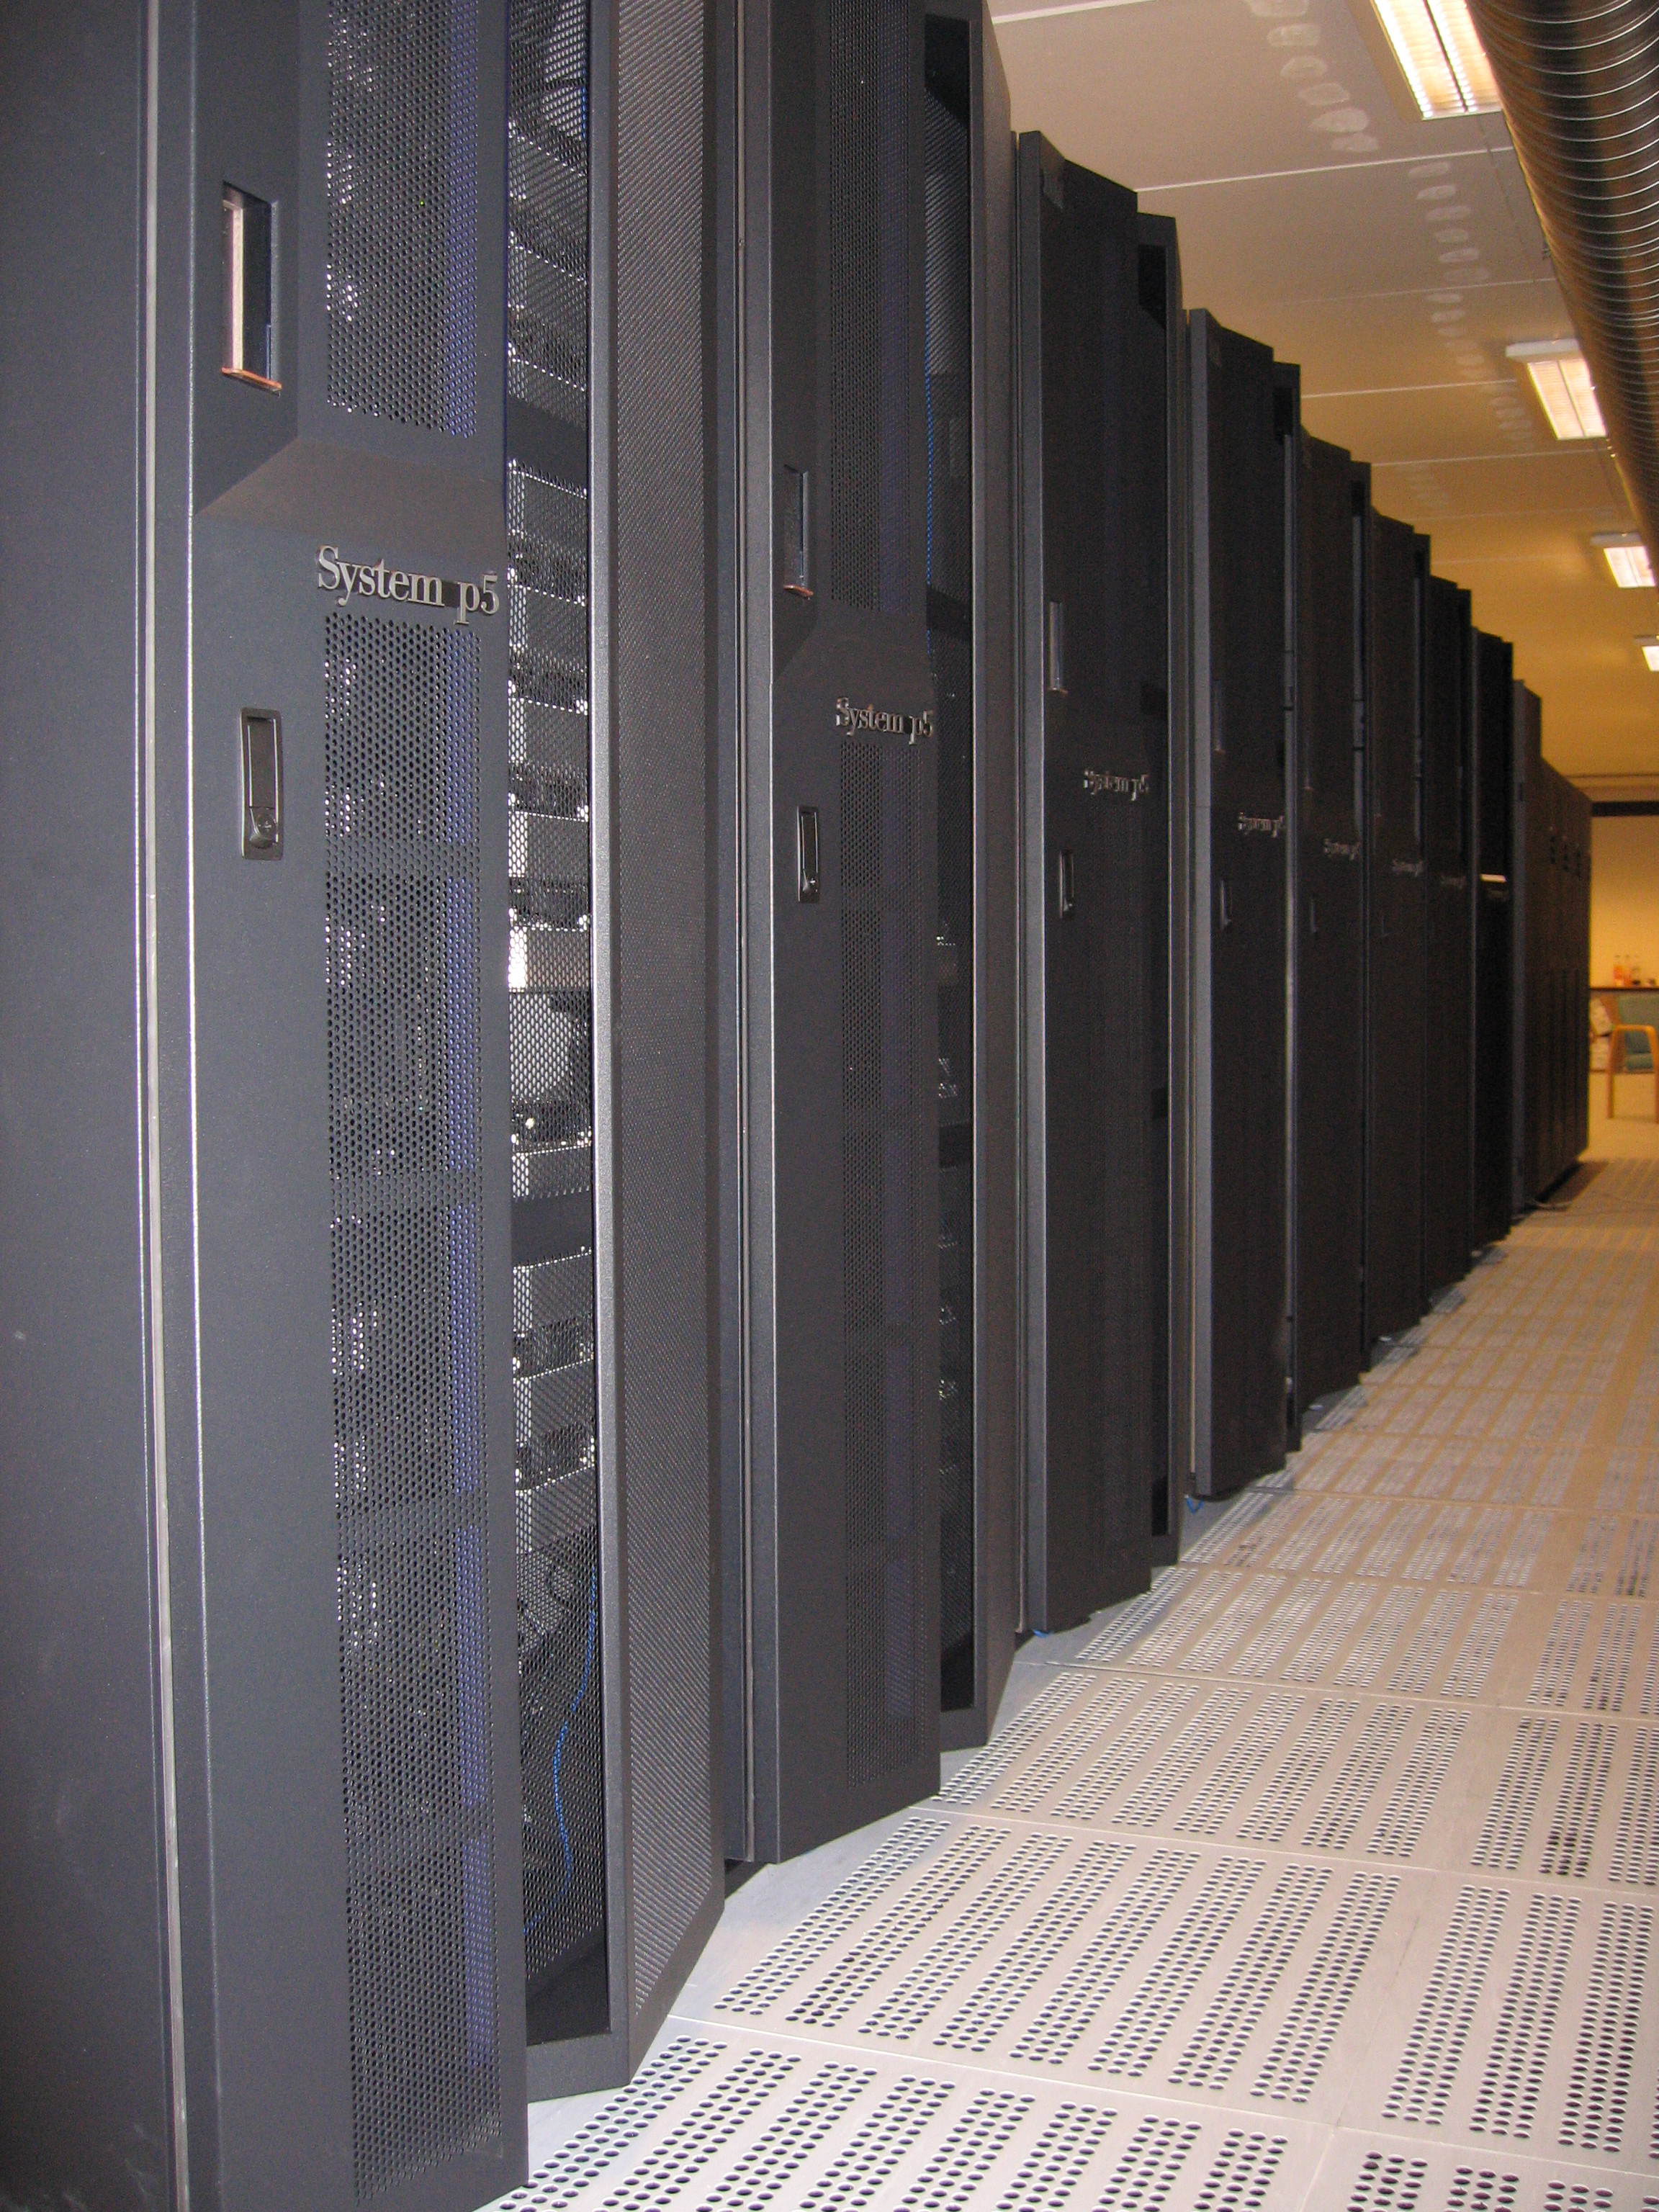
\includegraphics[width=6cm]{njord_1}
% \end{center}
% \end{frame}
% \begin{frame}\frametitle{An UNIX crash course - ssh, bash, build systems (CMake)}
% \begin{center}
% 
\includegraphics[width=6cm]{crash}
% \end{center}
% \end{frame}
% \begin{frame}\frametitle{An introduction to distributed memory programming
%                          using the MPI library.}
% \begin{center}
% \texttt{  node 0 :   Hello, world}\\
% \texttt{  node 1 :   Hello, world}\\
% \texttt{  node 3 :   Hello, world}\\
% \texttt{  node 2 :   Hello, world}
% \end{center}
% \begin{center}
% 
\includegraphics[width=3cm]{open-mpi-logo}
% \end{center}
% \end{frame}

% \begin{frame}\frametitle{An introduction to shared memory programming
%                          using the OpenMP standard.}
% \begin{center}
% \texttt{\#pragma omp parallel for schedule(static)}
% \end{center}
% \begin{center}
% 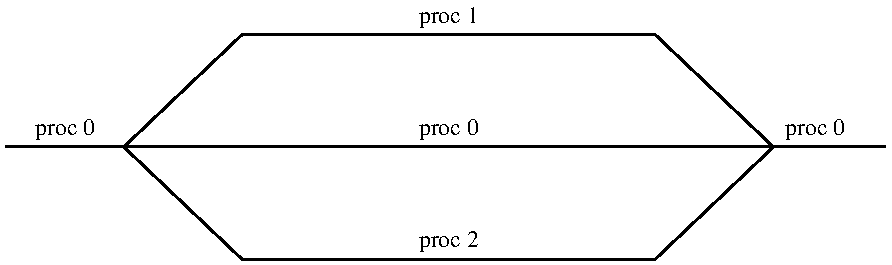
\includegraphics[width=4cm]{openmp}
% \end{center}
% \end{frame}

% \begin{frame}\frametitle{An introduction to heterogenous (GPU) computing
%                          using the CUDA standard.}
% \begin{center}
%   \texttt{int row = blockIdx.x*blockDim.x+threadIdx.x;}
% \end{center}
% \begin{center}
% 
\includegraphics[width=4cm]{cuda}
% \end{center}
% \end{frame}

% \begin{frame}\frametitle{A short introduction to parallel I/O using MPI-IO}
%   \begin{center}
%     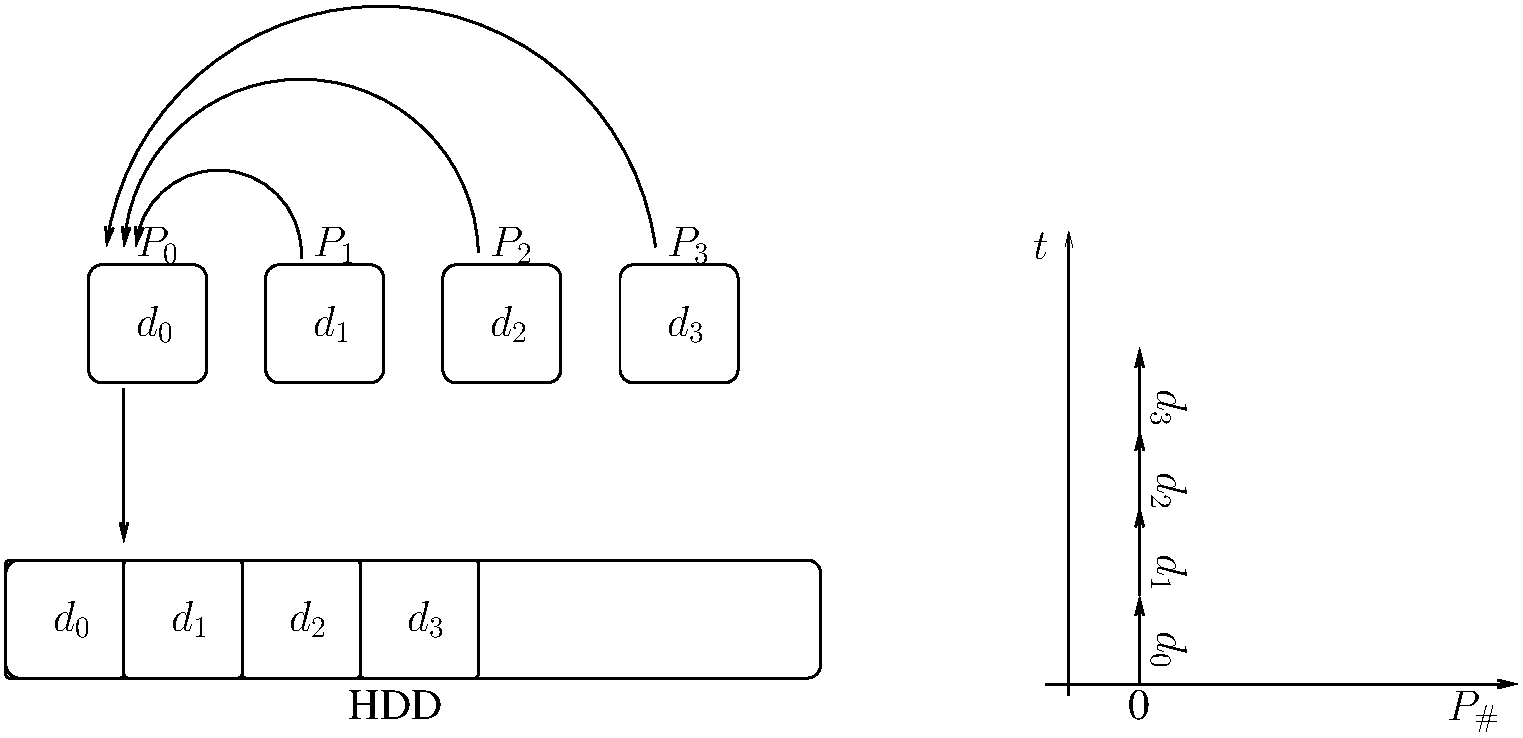
\includegraphics[width=8cm]{serial}
%   \end{center}
% \end{frame}

% \begin{frame}\frametitle{The Poisson problem: Discretization using finite difference methods}
% \[
%   \begin{split}
%     -\nabla^2 u &= f \\
%     u_{\partial\Omega} &= g
%   \end{split}
% \]
% \begin{center}
% 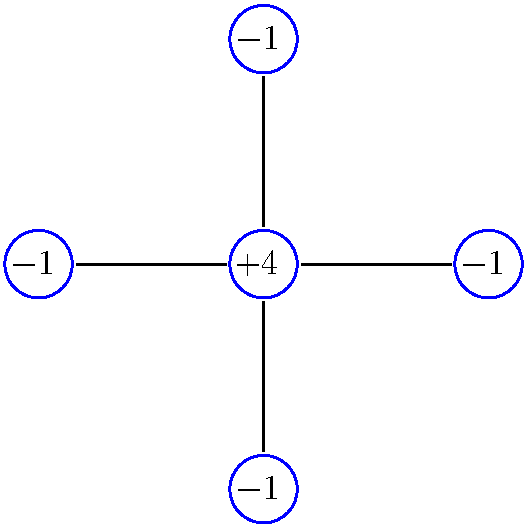
\includegraphics[width=4cm]{FivePointStencil}
% \end{center}
% \end{frame}
% \begin{frame}\frametitle{The Poisson problem: fast diagonalization methods}
% \underline{\textbf{Step 1)}}

% \begin{equation}
%   \underline{{\widetilde{G}}} = \underline{Q}^T \,\underline{G}\, \underline{Q} \qquad \longrightarrow \qquad \mathcal{O}(n^3) \text{ operations}.
% \end{equation}

% \underline{\textbf{Step 2)}}

% \begin{equation}
%   \widetilde{u}_{i,j} = \frac{\widetilde{g}_{i,j}}{\lambda_i + \lambda_j} \qquad \longrightarrow \qquad \mathcal{O}(n^2) \text{ operations}.
% \end{equation}

% \underline{\textbf{Step 3)}}

% \begin{align}
%   \underline{U} = \underline{Q} \,\underline{\widetilde{U}} \,\underline{Q}^T \qquad \longrightarrow \qquad \mathcal{O}(n^3) \text{ operations}. \\ \nonumber
% \end{align}
% \end{frame}

% \begin{frame}\frametitle{The conjugate gradient method}
%   \begin{center}
%     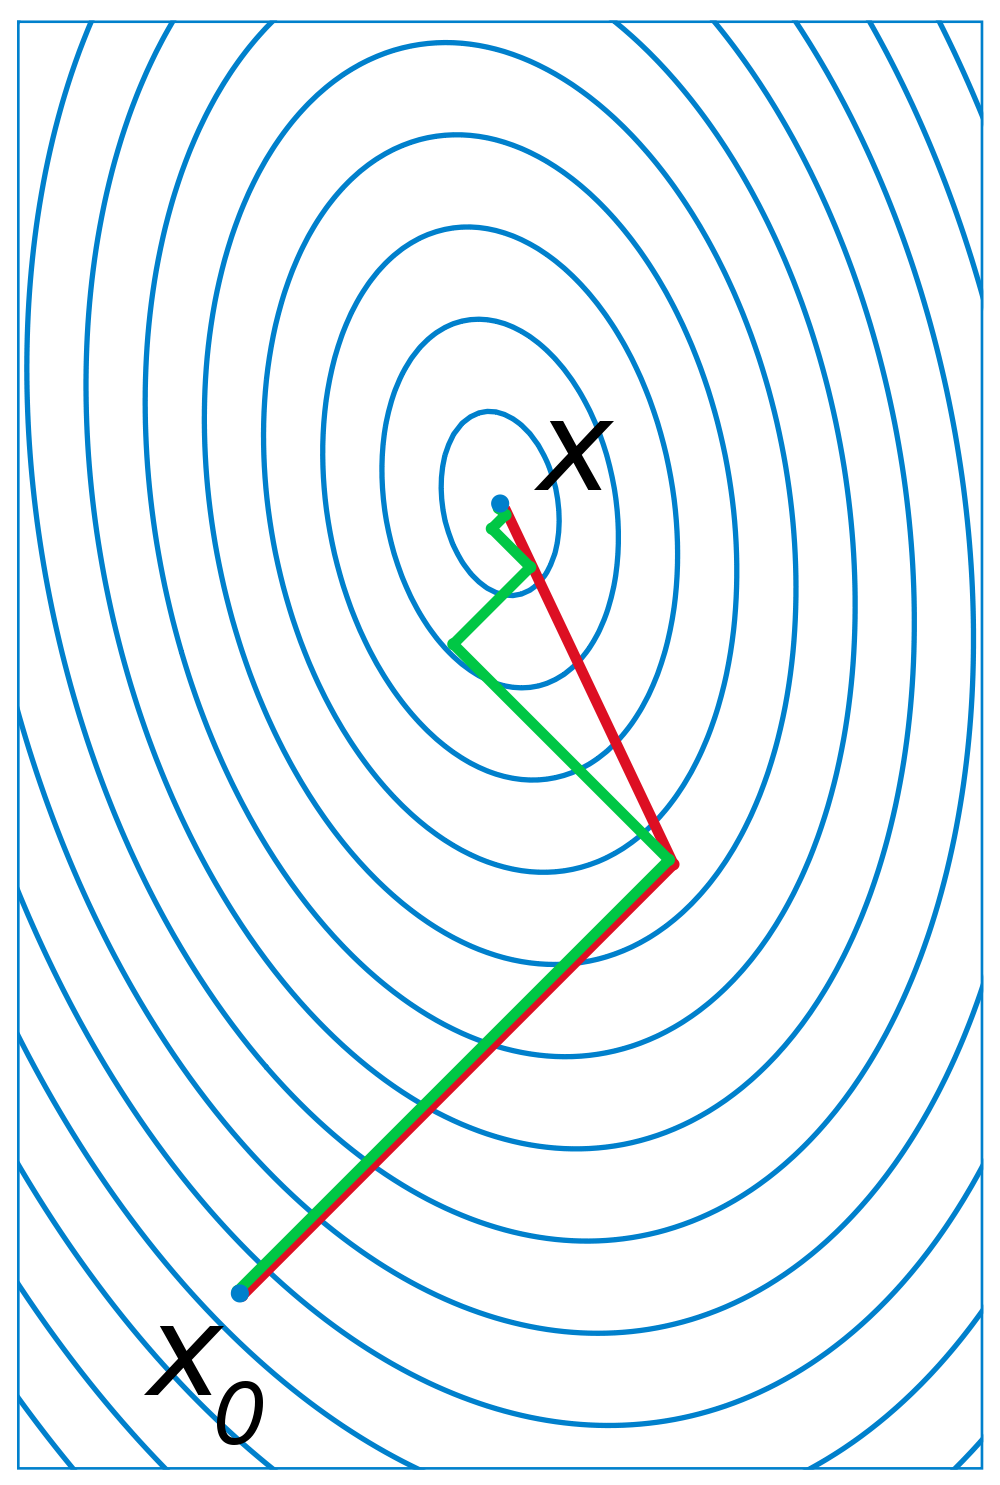
\includegraphics[width=4cm]{cg}
%   \end{center}
% \end{frame}

% \begin{frame}\frametitle{Parallel solution of a Poisson problem using
%                          matrix-free cg iterations and domain decomposition}
%   \begin{center}
%     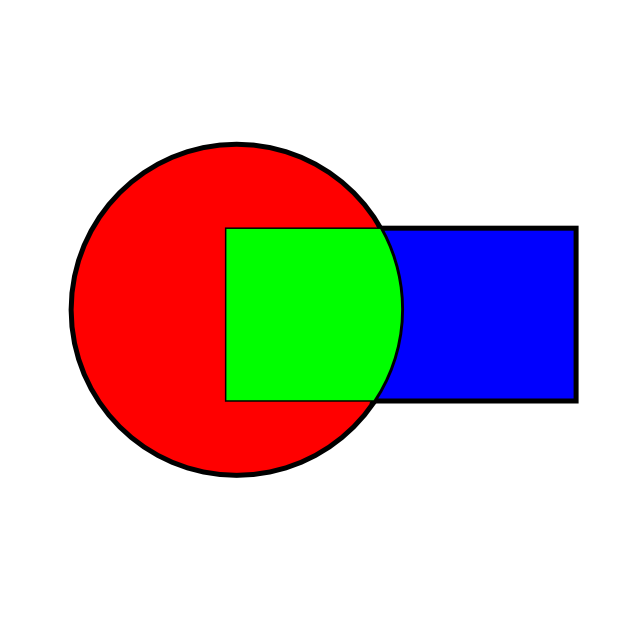
\includegraphics[width=8cm]{dd}
%   \end{center}
% \end{frame}

% \end{document}
